%%%%%%%%%%%%%%%%%%%%%%%%%%%%%%%%%%%%%%%%%%%%%%%%%%%
%% P3: Phenomenology of Particle Physics                         
%%
%% Author:  André Rubbia                   		 
%%
%% Figure 5.5 Angle in the laboratory frame vs. angle in the center-of-mass.
%%
%% This work is licensed under the Creative Commons Attribution 4.0 International License. 
%% To view a copy of this license, visit http://creativecommons.org/licenses/by/4.0/ or 
%% send a letter to Creative Commons, PO Box 1866, Mountain View, CA 94042, USA.
%%
%%%%%%%%%%%%%%%%%%%%%%%%%%%%%%%%%%%%%%%%%%%%%%%%%%%

\documentclass[a4paper,10pt]{article}

\usepackage[T1]{fontenc}
\usepackage[utf8]{inputenc}
\usepackage{lmodern}
\usepackage[labelfont=bf]{caption}
\usepackage{upgreek}

\usepackage{tikz}
\usepackage{pgfplots}
\pgfplotsset{compat=1.17}
\usepgfplotslibrary{ternary}
\usepgfplotslibrary{fillbetween}
\usepgfplotslibrary{external}

\def\d{\mathrm{d}}

\begin{document}

%%%%%%%%%%%%%%%%   FIGURE  %%%%%%%%%%%%%%%%%%%%%%%%%%%%%%
\begin{figure}[htb]
\begin{center}
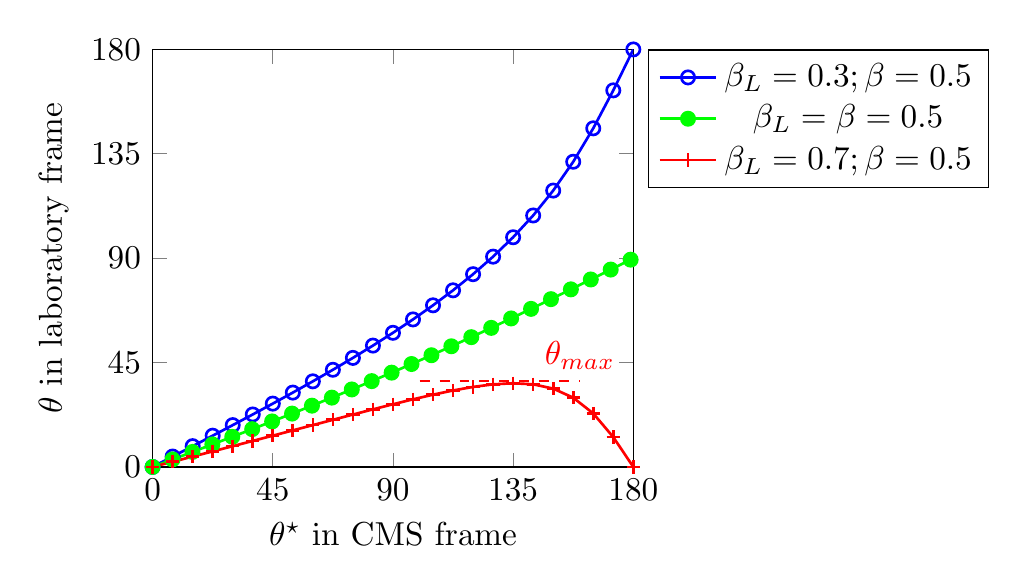
\begin{tikzpicture}[scale=1.2]
\begin{axis}[width=0.55\textwidth,height=6cm, xmin=0, xmax=180, xtick={0,45,90,135,180},
	ytick={0,45,90,135,180},ymin=0, ymax=180,
	xlabel=$\theta^\star$ in CMS frame,
	ylabel=$\theta$ in laboratory frame,
	legend entries={$\beta_L=0.3; \beta=0.5$,
	$\beta_L=\beta=0.5$,
	$\beta_L=0.7; \beta=0.5$},
	legend pos = outer north east]
	\addplot[domain=0:180,blue,thick, mark=o] {atan2(sqrt(1-(0.3)^2)*sin(x),(0.3/0.5+cos(x)))};
	\addplot[domain=0:179,green,thick, mark=*] {atan2(sqrt(1-(0.5)^2)*sin(x),(1+cos(x)))};
	\addplot[domain=0:180,red,thick, mark=+] {atan2(sqrt(1-(0.7)^2)*sin(x),(0.7/0.5+cos(x)))};
	\draw[dashed,red] (axis cs:100,37) -- (axis cs:160,37) node[above] {$\theta_{max}$};
\end{axis}
\end{tikzpicture}
\caption{Angle in the laboratory frame vs. angle in the center-of-mass for the three
cases (a) $\beta_L <\beta$, (b) $\beta_L =\beta$, and (c) $\beta_L>\beta$.}
\end{center}
\end{figure}
%%%%%%%%%%%%%%%%   END FIGURE  %%%%%%%%%%%%%%%%%%%%%%%%%%%%%%
%

\end{document}
